\documentclass{article}

\usepackage[utf8]{inputenc}
\usepackage{amsfonts}
\usepackage{amsmath}
\usepackage{booktabs}
\usepackage{color}
\usepackage{colortbl}
\usepackage{dirtytalk}
\usepackage{graphicx}
\usepackage{hyperref}
\usepackage{listings}
\usepackage[square,sort,comma,numbers]{natbib}
\usepackage{url}
\usepackage{semantic}
\usepackage{tikz}
\usepackage{todonotes}

\lstdefinestyle{Racket}{
  language=Lisp,
  basicstyle=\ttfamily,
  otherkeywords={\#lang,define,match,let,:,->,lambda,struct,define-type,car,cdr},
  identifierstyle=\color{pink!60!blue},
  keywordstyle=\color{blue!50!black},
  stringstyle=\color{green!50!black},
  commentstyle=\color{pink!60!black}
}

\lstdefinestyle{Java}{
  language=Java,
  basicstyle=\ttfamily,
  identifierstyle=\color{orange!40!black},
  keywordstyle=\color{blue!50!black},
  stringstyle=\color{green!50!black},
  commentstyle=\color{blue!50!grey}
}

\lstset{
  style=Racket
}

\usetikzlibrary{shapes.multipart, chains, positioning}
\tikzset{cons/.style n args=2{
    on chain,
    rectangle split,
    rectangle split horizontal,
    rectangle split parts=2,
    draw,
    anchor=center,
    text height=1.5ex,
    node contents={#1\nodepart{two}#2},
    join={by ->}
  }
}

\title{Lecture Notes:\\Functional Programming in Typed Racket}
\author{Florian Biermann \\\small{\texttt{fbie@itu.dk}} \\~}

\date{2016-06-17}

\begin{document}
\maketitle

\section{Sequential and Parallel Expressions}

Imagine you write this expression in Racket:

\begin{center}
  \lstinline{(+ 1 (+ 2 (+ 3 (+ 4 (+ 5 6)))))}
\end{center}


The Racket syntax already makes it clear how the corresponding abstract syntax tree (AST) looks like:

\begin{center}
  \begin{tikzpicture}[level distance=0.5cm]
    \node {\lstinline{+}}
    child {node {\lstinline{1}}}
    child {node {\lstinline{+}}
      child {node {\lstinline{2}}}
      child {node {\lstinline{+}}
        child {node {\lstinline{3}}}
        child {node {\lstinline{+}}
          child {node {\lstinline{4}}}
          child {node {\lstinline{+}}
            child {node {\lstinline{5}}}
            child {node {\lstinline{6}}}}}}};
  \end{tikzpicture}
\end{center}

The AST shows that there is a sequential dependency between each invocation of \lstinline{+}, which is the long spine going from the upper left to the lower right. If your program runs on a single core processor, this is a good solution. Today's modern processors however are multi-core processors. Can we change the expression to make use of more than one processor?

As it turns out, this is entirely possible. Consider the following expression instead:

\begin{center}
  \lstinline{(+ (+ 1 (+ 2 3)) (+ 4 (+ 5 6)))}
\end{center}

Note that we still use the same number of \lstinline{+} operations. It will compute the same number, because \lstinline{+} is an \emph{associative operation}. Associativity means that the order in which the operations are applied does not matter for the result, and therefore it holds that

\begin{center}
  \lstinline{(+ a (+ b c))} = \lstinline{(+ (+ a b) c)}
\end{center}

or

\begin{center}
  $a + (b + c) = (a + b) + c$
\end{center}

if you prefer mathematical notation. This is how the AST looks like for the reformulated expression:

\begin{center}
  \begin{tikzpicture}[level distance=.5cm]
    \tikzstyle{level 1}=[sibling distance=4.8cm]
    \tikzstyle{level 2}=[sibling distance=2.4cm]
    \tikzstyle{level 3}=[sibling distance=2.4cm]
    \node {\lstinline{+}}
    child {node {\lstinline{+}}
      child {node {\lstinline{1}}}
      child {node {\lstinline{+}}
        child {node {\lstinline{2}}}
        child {node {\lstinline{3}}}
      }
    }
    child {node {\lstinline{+}}
      child {node {\lstinline{4}}}
      child {node {\lstinline{+}}
        child {node {\lstinline{5}}}
        child {node {\lstinline{6}}}
      }
    };
  \end{tikzpicture}
\end{center}

Now, instead of a tree with a long spine, we have a somewhat balanced binary tree. The branches of trees are independent from each other, otherwise the tree would be a cyclic graph. We can make use of this independence, because independent sub-trees means independent calculations and independent calculations means that there is an opportunity for parallelism!

We can reformulate any sequential expression that calls the same function \lstinline{f} recursively if it holds that \lstinline{(f a (f b c))}~ = ~ \lstinline{(f (f a b) c)}, i.e. that \lstinline{f} is an associative operation:

\begin{center}
  \begin{tikzpicture}[level distance=.5cm]
    \tikzstyle{level 1}=[sibling distance=4.8cm]
    \tikzstyle{level 2}=[sibling distance=2.4cm]
    \tikzstyle{level 3}=[sibling distance=1.2cm]
    \node {\lstinline{f}}
    child {node {\lstinline{f}}
      child {node {\lstinline{f}}
        child {node {\dots}}
        child {node {\dots}}
      }
      child {node {\lstinline{f}}
        child {node {\dots}}
        child {node {\dots}}
      }
    }
    child {node {\lstinline{f}}
      child {node {\lstinline{f}}
        child {node {\dots}}
        child {node {\dots}}
      }
      child {node {\lstinline{f}}
        child {node {\dots}}
        child {node {\dots}}
      }
    };
  \end{tikzpicture}
\end{center}

\section{Sequential and Parallel Functions}

Take a look at the code for sequentially mapping a function over the standard cons-list (or linked list) in Racket:

\begin{lstlisting}
(: seq-map (All (A B) (-> (-> A B) (Listof A) (Listof B))))
(define (seq-map f xs)
  (match xs
    ['() '()]
    [(cons x xs) (cons (f x) (seq-map f xs))]))
\end{lstlisting}

And here is a hypothetical call-tree for \lstinline{seq-map}:

\begin{center}
  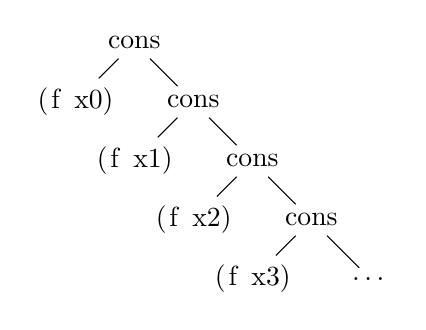
\begin{tikzpicture}[level distance=0.75cm]
    \node {\lstinline{cons}}
    child {node {\lstinline{(f x0)}}}
    child {node {\lstinline{cons}}
      child {node {\lstinline{(f x1)}}}
      child {node {\lstinline{cons}}
        child {node {\lstinline{(f x2)}}}
        child {node {\lstinline{cons}}
          child {node {\lstinline{(f x3)}}}
          child {node {\dots}}}}};
  \end{tikzpicture}
\end{center}

Again, you see the for sequential computations typical long spine in the tree. Can we turn this sequential function into a parallel function?

Exercise: try to do it now!

You will quickly see that there is no way to efficiently combine two lists without adding new sequential operations. This is because the \lstinline{cons} constructor is of type \lstinline{(All A (-> A (Listof A)))}. It does not know how to combine two lists. Therefore, we cannot write a parallel version of \lstinline{seq-map} on lists. This becomes even more obvious if you visualize the linked list':

\begin{center}
  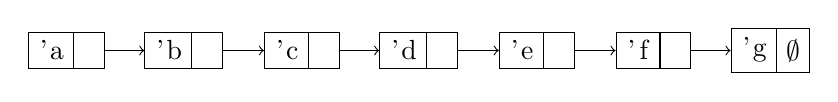
\begin{tikzpicture}[start chain=going right]
    \node (a) [cons={\lstinline{'a}}{}];
    \node (b) [cons={\lstinline{'b}}{}];
    \node (c) [cons={\lstinline{'c}}{}];
    \node (d) [cons={\lstinline{'d}}{}];
    \node (e) [cons={\lstinline{'e}}{}];
    \node (f) [cons={\lstinline{'f}}{}];
    \node (g) [cons={\lstinline{'g}}{$\emptyset$}];
  \end{tikzpicture}
\end{center}

What can we do instead? We can create a new data structure that supports parallelism by its very nature. How would such a data structure look like? The parallel expression for the sum from 1 to 6 was a binary tree, so let's try to use a tree to represent our list. We call it \lstinline{CatListof A}, where \emph{cat} is short for concatenation:

\begin{lstlisting}
(define-type (CatListof A) (U (leaf A)
                              (cat A)))
(struct (A) leaf ([a : A]))
(struct (A) cat  ([l : (CatListof A)]
                  [r : (CatListof A)]))
\end{lstlisting}

\lstinline{(leaf a)} produces a singleton \lstinline{(CatListof A)}. \lstinline{(cat l r)} concatenates two \lstinline{(CatListof A)} instances and produces a new instance of \lstinline{(CatListof A)}. Here is an illustration of an instance of \lstinline{(CatListof A)} where circles are \lstinline{cat} instances and rectangles are \lstinline{leaf} instances:

\begin{center}
  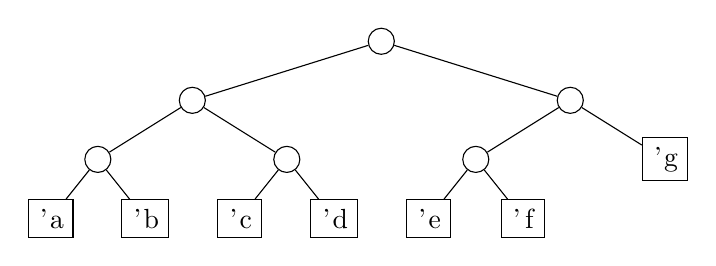
\begin{tikzpicture}[level distance=0.75cm]
    \tikzstyle{level 1}=[sibling distance=4.8cm]
    \tikzstyle{level 2}=[sibling distance=2.4cm]
    \tikzstyle{level 3}=[sibling distance=1.2cm]
    \node [circle, draw] {}
    child {node [circle, draw] {}
      child {node [circle, draw] {}
        child {node [rectangle, draw] {\lstinline{'a}}}
        child {node [rectangle, draw] {\lstinline{'b}}}
      }
      child {node [circle, draw] {}
        child {node [rectangle, draw] {\lstinline{'c}}}
        child {node [rectangle, draw] {\lstinline{'d}}}
      }
    }
    child {node [circle, draw] {}
      child {node [circle, draw] {}
        child {node [rectangle, draw] {\lstinline{'e}}}
        child {node [rectangle, draw] {\lstinline{'f}}}
      }
      child {node [rectangle, draw] {\lstinline{'g}}}
    };
  \end{tikzpicture}
\end{center}

Now, we can implement a map-function on \lstinline{(CatListof A)} instances:

\begin{lstlisting}
(: cat-map
  (All (A B) (-> (-> A B) (CatListof A) (CatListof B))))
(define (cat-map f xs)
  (match xs
    [(leaf x) (leaf (f x))]
    [(cat l r) (cat (cat-map f l)
                    (cat-map f r))]))
\end{lstlisting}

This is still not parallel. However, the only way we can write a map-function for \lstinline{(CatListof A)} produces a call-tree that bears a \emph{possibility for parallelism}:

\begin{center}
  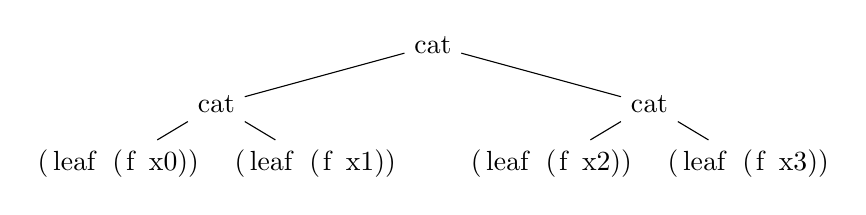
\begin{tikzpicture}[level distance=0.75cm]
    \tikzstyle{level 1}=[sibling distance=5.5cm]
    \tikzstyle{level 2}=[sibling distance=2.5cm]
    \node {\lstinline{cat}}
    child {node {\lstinline{cat}}
      child {node {\lstinline{(leaf (f x0))}}}
      child {node {\lstinline{(leaf (f x1))}}}}
    child {node {\lstinline{cat}}
      child {node {\lstinline{(leaf (f x2))}}}
      child {node {\lstinline{(leaf (f x3))}}}};
  \end{tikzpicture}
\end{center}

\section{Parallelism in Racket}

Racket and Typed Racket use a fork/join style model of parallel computations. Fork is called \lstinline{future} and join is called \lstinline{touch}. We can use it to compute two functions in parallel as follows:

\begin{lstlisting}
(: in-parallel
  (All (A B C) (-> (-> A B) (-> A C) A (Pairof B C))))
(define (in-parallel f g x)
  (let ([fx (future (lambda () (f x)))]
        [gx (g x)])
    (cons (touch fx) gx)))
\end{lstlisting}

Here, the function the function \lstinline{g} is computed on the same thread and \lstinline{f} is computed on a different thread.When you call \lstinline{future} with a lambda expression, Racket creates a new object of type \lstinline{(Futureof A)}. This is a representation of an ongoing computation (i.e. the lambda expression) which possibly runs in parallel. If and on which processor core this future is computes is determined by the built-in scheduler. There is no need to explicitly create and manage threads in Racket.

In order to get the computed value, you need to synchronize the thread that wants to read the value with the thread that computes the value. This you do by calling \lstinline{touch} with the instance of \lstinline{(Futureof A)} from which you want to retrieve the value. If the thread that was computing the future is already done, the thread that is reading the value will just continue. If the future is not yet computed however, the reading thread will block until the computation is done.

This are the types of \lstinline{future} and \lstinline{touch}:

\begin{lstlisting}
  (: future (All (A) (-> (-> A) (Futureof A))))
  (: touch  (All (A) (-> (Futureof A) A)))
\end{lstlisting}

\section{Truly Parallel Functions}

Let us return to implementing a parallel version of a map-function for \lstinline{(CatListof A)}. We now have all the tools we need: a data-structure already laid out for parallelism and a way to express parallel computations in the language. So let's look at how the code for \lstinline{cat-map} looks like if we apply \lstinline{future} and \lstinline{touch}:

\begin{lstlisting}
(: par-map
  (All (A B) (-> (-> A B) (CatListof A) (CatListof B))))
(define (par-map f xs)
  (match xs
    [(leaf x) (leaf (f x))]
    [(cat l r)
       (let ([fl (future ;; Map l in parallel.
                   (lambda () (par-map f l)))]
             [fr (future ;; Map r in parallel.
                   (lambda () (par-map f r)))])
         (cat (touch fl) (touch fr)))]))
\end{lstlisting}

As you can see, we keep the overall structure of the function. The base-case for leaves remains completely untouched. Notice that the types of \lstinline{cat-map} and \lstinline{par-map} are identical. The difference is that, instead of calling \lstinline{par-map} recursively directly, we wrap the recursive call in a lambda-expression which we pass to the \lstinline{future} constructor. After we have created a future for the left and the right sub-tree of the list, we wait for both computations using \lstinline{touch} and then we combine the two resulting lists using \lstinline{cat}.

We call parallelism on aggregate data structures \emph{data-parallelism}, because the parallelism stems from the fact that we apply the same function to many different inputs in parallel.

By creating a new future at each node, we make sure that we exploit as much parallelism as possible. Also, we do not need to worry about how many threads we want to launch or how we want to chunk up the data, because Racket's scheduler takes care of that automatically. This does not come for free, though. Creating many futures for small trees might outweigh the benefit of parallelization, maybe even makes the operation slower.

\section{Limiting Parallelism with Ropes}

If the size of the tree is too small, then the overhead of constructing \lstinline{future}s dominates the run-time cost. We can handle this problem by using lists as leaves instead of scalar values to limit the degree of parallelism for small input sizes. We can use a data structure called a \emph{Rope}, which is a binary tree with sequential lists (or arrays) as leaves:

\begin{lstlisting}
(define-type (Ropeof A) (U (leaf A) (cat A)))
(struct (A) leaf ([as : (Listof A)]))
(struct (A) cat  ([l  : (Ropeof A)]
                  [r  : (Ropeof A)]))
\end{lstlisting}

We need to define a value $s_{\max}$ that limits the length of the leaf arrays. Here is an illustration of such a rope, where the $s_{\max} = 3$:

\begin{center}
  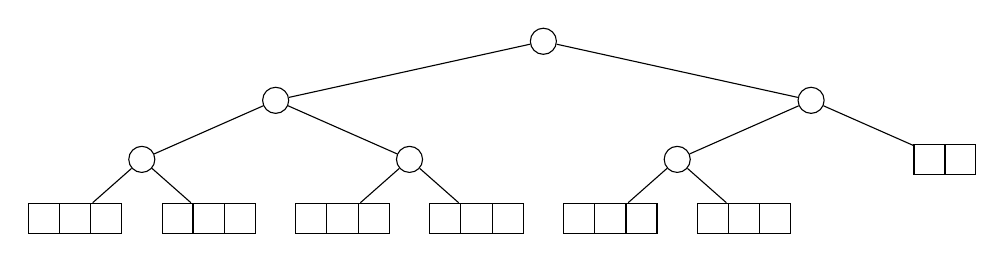
\begin{tikzpicture}[level distance=0.75cm]
    \tikzstyle{level 1}=[sibling distance=6.8cm]
    \tikzstyle{level 2}=[sibling distance=3.4cm]
    \tikzstyle{level 3}=[sibling distance=1.7cm]
    \node [circle, draw] {}
    child {node [circle, draw] {}
      child {node [circle, draw] {}
        child {node [rectangle split, rectangle split horizontal, rectangle split parts=3, draw] {}}
        child {node [rectangle split, rectangle split horizontal, rectangle split parts=3, draw] {}}
      }
      child {node [circle, draw] {}
        child {node [rectangle split, rectangle split horizontal, rectangle split parts=3, draw] {}}
        child {node [rectangle split, rectangle split horizontal, rectangle split parts=3, draw] {}}
      }
    }
    child {node [circle, draw] {}
      child {node [circle, draw] {}
        child {node [rectangle split, rectangle split horizontal, rectangle split parts=3, draw] {}}
        child {node [rectangle split, rectangle split horizontal, rectangle split parts=3, draw] {}}
      }
      child {node [rectangle split, rectangle split horizontal, rectangle split parts=2, draw] {}}
    };
  \end{tikzpicture}
\end{center}

Choosing the a good value for $s_{\max}$ is important. If we set $s_{\max}$ too low, our algorithms will probably create excessively many \lstinline{future} instances, but if we set $s_{\max}$ too high, we will not expose enough parallelism to gain any performance benefits.

Finding a good value for $s_{\max}$ depends a lot on the application. Do you expect to map mostly long-running functions on your collection? Will this function have roughly the same run-time for each input or will it vary heavily? There are many factors that you need to consider.

How do we implement \emph{map} for this data structure? It is actually quite similar to our \lstinline{CatListof A} implementation. But because the leaves of the rope are not scalar values but another collection data type, we must rely on using also a higher-order \emph{map} function for this data structure. Since we use the built-in \lstinline{cons} list, we can simply use the default \lstinline{map} function that comes with it:

\begin{center}
\begin{lstlisting}
(: rope-map
  (All (A B) (-> (-> A B) (Ropeof A) (Ropeof B))))
(define (rope-map f rope)
  (match rope
    [(leaf as) (leaf (map f as))]
    [(cat l r) (cat (rope-map f l)
                    (rope-map f r))]))
\end{lstlisting}
\end{center}

This is a straight-forward implementation of \emph{map} on ropes. The base case for leaves does not apply the function \lstinline{f} directly. Instead, it calls \lstinline{map} on \lstinline{cons} lists and passes \lstinline{f} on to the call.

The recursive case for \lstinline{cat} simply decomposes the rope into its subtrees and calls itself recursively just as we did it for the \lstinline{CatListof A}.

We can now proceed and write a parallel version of this function. All we need to do is, again, to wrap the recursive calls to \lstinline{rope-map} in a lambda expression and pass it to \lstinline{future}. We call this version of \lstinline{rope-map} simply \lstinline{rope-pmap}, where p stands for ``parallel''. Notice again that the types of both functions are the same. Notice furthermore that we again do not change the base case for \lstinline{leaf}, because here, we explicitly prefer sequential execution:

\begin{lstlisting}
(: rope-pmap
  (All (A B) (-> (-> A B) (Ropeof A) (Ropeof B))))
(define (rope-pmap f rope)
  (match rope
    [(leaf as) (leaf (map f as))]
    [(cat l r) (let [(l0 (future (lambda ()
                                   (rope-pmap f l))))
                     (r0 (future (lambda ()
                                   (rope-pmap f r))))]
                 (cat (touch l0) (touch r0)))]))
\end{lstlisting}

If we want to proceed to parallelize more functions on ropes, we simply can first implement the simplest sequential version of the function that we can think of. Then, in the next step, we can simply wrap the recursive call in a lambda expression and pass it to a call to \lstinline{future}. We do not need to worry about thread safety, because the sub-trees are completely disjoint, so the computations will not interfere with each other.

Here is another example, the implementations for the rope versions of \emph{reduce}, namely \lstinline{rope-reduce} and \lstinline{rope-preduce}:

\begin{lstlisting}
(: rope-reduce
  (All (A) (-> (-> A A A) (Ropeof A) A)))
(define (rope-reduce f rope)
  (match rope
    [(leaf as) (list-reduce f as)]
    [(cat l r) (f (rope-reduce f l)
                  (rope-reduce f r))]))

(: rope-preduce
  (All (A) (-> (-> A A A) (Ropeof A) A)))
(define (rope-preduce f rope)
  (match rope
    [(leaf as) (list-reduce f as)]
    [(cat l r) (let [(l0 (future (lambda ()
                                   (rope-preduce f l))))
                     (r0 (future (lambda ()
                                    (rope-preduce f r))))]
                 (f (touch l0) (touch r0)))]))
\end{lstlisting}

Does this mean that we can parallelize \emph{all} higher-order functions that we can think of? It turns out that this is not the case. For instance, the general \emph{fold} function is of type $(B \rightarrow A \rightarrow B) \rightarrow B \rightarrow [A] \rightarrow B$, where $[A]$ denotes a collection of values of type $A$. We can write this type in Typed Racket for \lstinline{cons} list as \lstinline{(All (A B) (-> (-> B A B) B (Listof A) B))}.

We have learned that we can parallelize functions that are \emph{associative}. Therefore, in order to parallelize \emph{fold}, we must show that \lstinline{f} is commutative. If you look at its type, it becomes clear that it is not. Let us assume that we have a rope with a left and a right subtree. If we compute \emph{fold} for the left side and for the right side, following the definition of \emph{fold}, we end up with two values for each side, both of type $B$. But our function $f$ is of type $B \rightarrow A \rightarrow B$, which means we do not know how to combine two values of type $B$.

Therefore, we cannot parallelize \emph{fold} unless we add a second function parameter of type $B \rightarrow B \rightarrow B$. It turns out, that this is not necessary, because we can instead use \emph{map} and \emph{reduce} to achieve the same result.

\end{document}
